\section{Caracterizacion de un instrumento}

\subsection{Extracci\'on de Features}

Hoy se encuentran muchos descriptores de bajo nivel basados en el contenido espectral usados en este campo de investigación. Para intentar determinar el timbre de los instrumentos usamos cuatro: Zero Crossing Rate, Spectral Rolloff, Spectral Centroid, Spectral Flatness.

\begin{itemize}
    \item \textit{Zero-Crossing Rate:}  es la velocidad en la que el signo de una señal cambia entre positivo y negativo. Este feature suele dar buenos resultados para clasificar instrumentos percusivos.
        
    \item \textit{Spectral Rolloff:} es una medida de la forma de la señal. Se define para cada muestra como la frecuencia central para un bin del espectrograma de modo que al menos el 85\% de la energía del espectro en esta muestra está contenido en este bin y los de abajo. Esto se puede utilizar para, por ejemplo, aproximar la frecuencia máxima (o mínima) ya que mide la frecuencia donde se concentra un porcentaje de la distribución de magnitud.
        
    \item \textit{Audio Spectrum Centroid:} es una medida utilizada en el procesamiento digital de señales para caracterizar un espectro. Indica dónde está el centro de masa del mismo. Perceptualmente tiene una fuerte correlación con la impresión del brillo de un sonido.
        
    \item \textit{Audio Spectrum Flatness:} o el coeficiente de tonalidad, es otra medida del procesamiento de señales que sirve para caracterizar el espectro de un audio. Se mide típicamente en decibeles y provee una forma para cuantificar que tan tonal es un sonido, contrapuesto a que tan parecido al ruido es.
\end{itemize}

\subsection{Modelo}
\label{sec:modelo}


Parar el modelo usamos la \textit{factorización no negativa de matrices} (En adelante NMF). Esto es, dada una matriz no negativa $V$ de $n x m$ (m vectores de n dimenciones), es posible encontrar matrices no negativas $W$ y $H$ tal que
\begin{center}
    $V \approx WH$
\end{center}
donde $W$, de la forma $n x r$, contiene una base de vectores y $H$, de la forma $r x m$, contiene los pesos necesarios para aproximar la correspondiente columnas de $V$. En particular, $r$ se elige de manera arbitraria. Usualmente es bueno tomar un $r$ tal que $(n+m)r < nm$ de manera que la matriz resultante sea una versi\'on compresa de la original.
        
\subsection{Procesamiento de datos y experimentos}

\subsubsection{Dataset}

El set de sonidos utilizados incluyó platillos, violines, flautas, trombones, guitarra y trompetas, con apróximadamente 70 muestras de cada uno, todas del mismo largo y discretizadas usando 44.1 kHz de sampling rate. De estas tomamos un 10\% para test y el resto para entrenamiento. Por un lado podemos distinguir entre estos instrumentos aquellos que son percutidos -platillos y al ser cuerda percutida, la guitarra- de los que no, y los que son no-tonales -los platillos- de los tonales -el resto-.

A su vez las familias clásicas basadas en los descriptores de alto nivel los distinguen en cuerdas: guitarra, violín; vientos: trompeta, trombón, flauta; percusión: platillos. En la familia de los vientos también se distingue entre los metales (trombón y trompeta) y las maderas (flauta).

Estas muestras son distintas notas únicas de cada instrumento, o golpes si se trata de un platillo, con varias articulaciones dependiendo de las posibilidades de cada instrumento. Por lo que cada archivo de audio corresponde a un único instrumento, ejecutando una sola nota.

\subsubsection{Método de Clasificaci\'on según features}

Extrayendo los features previamente dichos, generamos un vector de features $v_j$ por cada audio y con eso armamos la matriz $V$ donde cada $v_j$ representa una columna de la misma. Además, al saber de qué instrumento es cada audio guardamos un vector $l$ con los labels de cada columna de $V$.

El entrenamiento del modelo consiste en aplicar NMF a $V$ para calcular $W$ y $H$. Luego calculamos la pseudo inversa $W^{-1}$.

Finalmente, para estimar un nuevo audio, generamos su vector de features $v_{test}$ y hacemos:

\begin{center}
    $h_{test} = W^{-1} v_{test}$
\end{center}

Solo nos queda matchear de alguna manera con los vectores $h$ que ya calculamos y estimar el label. Para esto usamos $KNN$ comparando $h_test$ contra los vectores columna de $H$ y consideramos los más cercanos a los que minimizan la \textit{distancia euclidea} entre ellos, esto es, los que minimizan la norma de la resta. Originalmente probamos maximizando \textit{Cosine Similarity}, pero esta medida no di\'o buenos resultados. 
    
\subsubsection{Evaluaci\'on}

Los parametros con los que experimentamos fueron por un lado las \textit{n componentes} sobre la factorizacion NMF, este ser\'ia el \textit{r} de la factorizacion (que tanto comprimimos los datos o que factores tenemos en cuenta). Por otro lado probamos con distintos valores de \textit{k} para los k vecinos mas cercanos. Finalmente maximizamos la performance en los valores \textbf{6} y \textbf{4} para \textbf{n\_components} y \textbf{k} correspondientemente. A continuacion mostramos los resultados obtenidos corriendo el modelo con estos parametros y comparando el uso de distintos features isolados para tratar de entender como estos impactan en la predicci\'on:

\begin{figure}[h!]
    \centering
    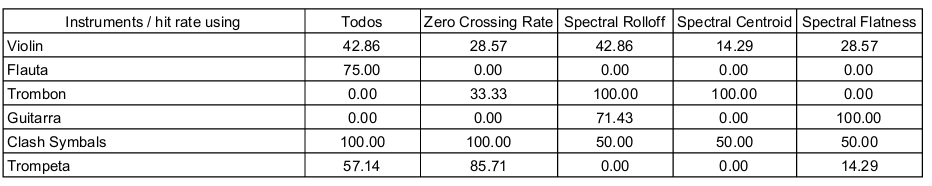
\includegraphics[scale=0.5]{Content/Figures/Comparacion_Features_Intrumentos.png}
    \caption{Resultados: Hit rate}
    \label{fig:resultados}
\end{figure}

\subsubsubsection{\textbf{Zero Crossing Rate}}

Era esperable que este descriptor de buenos resultados con instrumentos percusivos y en efecto los platillos fueron identificados correctamente en un 100\%.

\subsubsubsection{\textbf{Audio Spectral Roll-off}}

El descriptor de spectral roll-off arrojó buenos resultados para identificar las muestras de trombones y guitarras en menor medida.

\subsubsubsection{\textbf{Audio Spectrum Centroid}}

Consideramos que el 'brillo' de un sonido es una de las formas más sencillas de caracterizar y diferenciar sonidos, la formalización de esta característica corresponde a una indicación de la cantidad de energía en las frecuencias más altas de un sonido y es lo que podemos medir mediante el centroide espectral.

Llevado este análisis a los instrumentos estudiados encontramos un buen grado de precisión para el trombón. Sin embargo, el resultado no tiene una buena correlación con los descriptores de alto nivel dado que el trombón pertenece a la misma familia que la trompeta (vientos y metales) y es de un registro más grave, por lo que si obtuvimos buenos resultados con el trombón, hubieramos esperado obtener aún mejores resultados con la trompeta, ya que al ser de la misma familia y de un registro más agudo, debería haber mejorado su predicción con respecto al brillo.

\subsubsubsection{\textbf{Audio Spectral Flatness}}

Cuantificar qué tan tonal es un sonido no debería permitir distinguir instrumentos cuando son todos tonales, en nuestro set el único que se diferencia en esta dimensión son los platillos, que al ser inarmónicos deberían presentar diferenciarse facilmente de los demás.

Sin embargo, este desriptor no fue suficiente para lograr identificar esta distinción, el grado de precisión que arrojaron las muestras de platillos sugieren que este descriptor no alcanza para evidenciar esta hipótesis. En cuanto a la precisión que obtuvimos al predecir con los samples de guitarras, podemos suponer que la cualidad tonal de los mismos resultó más homogénea para este instrumento que para el resto.

\subsubsubsection{\textbf{Todos los descriptores combinados}}

Combinando todos los descriptores obtuvimos buenos resultados para identificar platillos en nuestro set de muestras, esta identificación mejoró a la obtenida por los descriptores separados (a excepción de Zero Crossing Rate, que dio igual). Esta combinación también mejoró la identificación de flautas, con el hecho notable de que por separado ningún descriptor había mostrado buena precisión. También mejoró la identificación de violines, aunque la precisión sigue siendo baja (por debajo del 50\%).

En el resto de los instrumentos vimos caer la precisión entre combinar los descriptores y utilizarlos por separado. No podemos afirmar que estos descriptores sean igual de determinantes para cada instrumento, ni para cada familia de instrumento, tampoco que mientras más descriptores combinemos, mejores resultados obtengamos. Es posible que los descriptores elegidos sean relevantes para los instrumentos percusivos inarmónicos (como los platillos) y no para los armónicos o melódicos (el resto). Una continuación de este trabajo debería constatar estos resultados con otros instrumentos percusivos e incluir descriptores nuevos para probar si pueden distinguir aquellos que producen sonidos armónicos entre sí.

Asi, podemos ver como queda la matriz de confusion resultante:

\begin{figure}[h!]
    \centering
    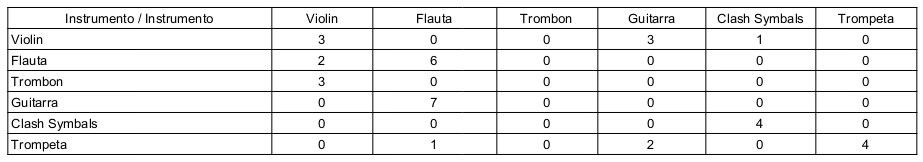
\includegraphics[scale=0.5]{Content/Figures/matriz-de-confusion.png}
    \caption{Matriz de Confusion entrenando con todos los features}
    \label{fig:my_label}
\end{figure}

Por lo que se muestra en la misma tiene bastante concentración en la diagonal para la flauta y clash cymbals mientras que para el resto de los instrumentos no hubo un gran desempeño. En particular todos los sonidos provenientes de las guitarras los clasificó como flautas pero se debe a que no analizamos tantos features. Con respecto a los violines su performance fue bastante buena ya que la gran mayoría de los sonidos los clasificó como violín o guitarra. Es decir las confusiones fueron sobre instrumentos de cuerda.